\documentclass[10pt]{article}
% for editing use
%\usepackage{lineno}
%\linenumbers
%\usepackage{endfloat}

% minimal packages here
\usepackage{booktabs}
\usepackage[noadjust]{cite}
\bibliographystyle{IEEEtran}
\usepackage[plain]{fancyref}
\renewcommand{\freffigname}{Fig.}
\renewcommand{\Freffigname}{Fig.} 
\renewcommand{\freftabname}{Table}
\renewcommand{\Freftabname}{Table}
\frefformat{plain}{\fancyrefeqlabelprefix}{(#1)} 
\Frefformat{plain}{\fancyrefeqlabelprefix}{(#1)} 
\usepackage{siunitx}
\usepackage{graphicx}
\usepackage{hyperref}
\hypersetup{%
	colorlinks=true,
	linkcolor=violet,
	urlcolor=blue,
	citecolor=blue,
	pdfauthor={Corwin Stites},
	pdftitle={Unmanned underwater vehicle mobile mesh networks: applications for hydrographic surveying},
	pdfsubject={weapons, robotics, and control engineering},
	pdfkeywords={UUV, mesh networks, hydrographic survey}}

% for editing use
\usepackage{color}
\definecolor{mygreen}{RGB}{28,172,0}
\definecolor{mylilac}{RGB}{170,55,241}
\usepackage[colorinlistoftodos]{todonotes}

% Bowman Scholar White Paper
\title{Unmanned underwater vehicle mobile mesh networks: applications for hydrographic surveying}
\author{Corwin W. Stites\thanks{Author is with the Department of Weapons, Robotics, and Control Engineering at the United States Naval Academy. Address for correspondence: \emph{m216468@usna.edu}}}
\date{February 5, 2020}

\begin{document}
\maketitle

\begin{abstract}
	Underwater surveying is a costly and time consuming endeavor. My proposed project would look into how a mobile mesh network could be applied to make hydrographic surveys more efficient and accurate. Such a network would consist of a group of sonar equipped Unmanned Underwater Vehicles (UUVs) connected via a mesh network actuated through an acoustic modem. The project would primarily focus on researching how nodes of the mesh network would communicate for best effect to accomplish fast hydrographic surveying of a predetermined area or fast location of an underwater target of interest. 
\end{abstract}
{\scriptsize\textbf{Keywords: } UUV, mesh networks, hydrographic survey}

\section{Midshipman Research Description}
Nearly 80\% of U.S. international trade moves through ports which require constant bathymetry to ensure the safe transit of vessels. Underwater surveying is critical to detecting changing conditions or obstructions that could be hazardous to navigation. 500,000 square miles of U.S. waters are deemed navigationally significant and must be regularly surveyed by the National Oceanic and Atmospheric Administration (NOAA). These surveys are typically carried out by a single ship or underwater vehicle operating in a search pattern. This process requires a large amount of time and resources and as a result the NOAA must prioritize which areas it surveys \cite{noaa2009hydrographic}.
	
The disappearance of Malaysia Airline Flight 370 in March of 2014 further illustrated the lack of surveying capabilities for large areas of ocean. Over 200,000 square kilometers were searched in two separate operations in an unsuccessful attempt to find the missing aircraft \cite{australia2018joint}. Another revelation from the search for MA 307 was the validation of UUV fleet technology. The company Ocean Infinity used its fleet of eight advanced surveying UUVs for the first time on a large scale. The fleet was able to search in a collaborative pattern, surveying areas much more quickly and efficiently than any other search asset \cite{economist2018fantastical}. This new application of fleet technology showed that UUV fleets prove more robust and efficient at surveying large areas. The individual bots in the fleet, while mostly autonomous, still required their search paths to be set by humans and still required periodic communication with the main ship via an acoustic modem \cite{haun2017ocean}. 	

There are possibilities to further streamline a fleet UUV system. Removing the need for operator route planning and ship communication would add an additional element of autonomy. This would be useful for operators trying to expand the size of a UUV fleet or trying to operate multiple fleets simultaneously. More numerous and larger fleets capable of being operated from one manned element would allow for even greater capabilities in searching for deep water objects and carrying out routine hydrographic surveying. A mesh network is a network in which individual assets in the group (called nodes) can communicate with each other cooperatively to function independent of outside control. Utilization of a mesh network could allow for these developments. With a mesh control algorithm, routes would not need to be planned by human operators. A search area could merely be given to the fleet and the mesh protocol could then plan the search patterns of individual assets. Furthermore, the mesh protocol could correct the course errors of individual assets via relative position to other nodes when a particular node’s dead reckoning goes off course. This means guidance from the ship would not be required. For this model, knowledge of predetermined UUV tasks would have to be built into each node to limit the information transmitted between nodes. 

The project I am proposing would focus primarily on the overall architecture of the mesh network. Specifically, this would mean selecting and implementing specific methods for relaying messages and algorithms for reconfiguration around network gaps. My project would address how these two factors can best be designed to meet a variety of constraints. In terms of the design of the mesh network’s protocol, the critical question is what method should be used in routing packets of data between nodes. There are two possibilities for this, flooding or routing. With flooding, packets of data are sent from one node to every other open link except the one from which the packet was received. This means all nodes functioning in the network will receive the packet with all nodes acting as both transmitters and receivers. The advantages of this protocol is that it is simple and robust. It is easy to implement and since packets travel through multiple routes, even with gaps in the network, it is almost guaranteed to arrive. The disadvantage lies in the fact that such a network wastes a large amount of bandwidth transmitting redundant messages and is vulnerable to distributed denial of service attacks. Additionally there are subsets of flooding such as simple flooding (Naive Flooding) and more selective flooding algorithms (Optimized Flooding) that would be tested \cite{zahn2009empirical}. Routing uses an algorithm which moves packets through a selected path of nodes to its destination. The packet determines a path and hops from one node to the next. There are also subsets of routing. Some protocols use pre planned routes for packets (Traditional Routing), and some determine a path as the packet transmits based on link quality (Opportunistic Routing)  \cite{hamraz2019wireless}. Since such a protocol has a set path, a self healing algorithm would have to be implemented to move packets around a gap in the event of a link failure. Once again there are various methods of self healing that would be tested \cite{trehan2019algorithms}.

The type of communication used at the transport layer will also have to be determined. The decision lies between UDP (User Datagram Protocol) or TCP (Transmission Control Protocol). TCP is considered much more reliable since it has the ability to check for and resend lost data packets as well as rearrange data packets into the correct sequence. However, this ability means higher latency times and demands higher data transmission quantities. UDP merely sends packets without checking for successful transmission. As a result, UDP has much lower associated latency times and transmission requirements but also has no guarantee of intact packet delivery. Less data overhead could be a significant advantage when using a relatively slow acoustic modem in a noisy underwater environment, however, simulation will determine if the amount of errors generated by a UDP protocol will be acceptable for the system to operate effectively. If UDP does not meet the system’s constraints, TCP must be considered instead \cite{rouse2019what}.

Using modeling and simulation on the MATLAB, NetworkX, and NS-3 platforms, various mesh algorithms would be tested under multiple constraints. The first constraint is the ability to transmit data in an underwater environment, most likely through an acoustic modem. Data rates will have to be within the capabilities of such a system. The second is reliability across a network of around 20 UUVs. The algorithm will have to be reliable and immune to specific node failure with a goal number of 20 nodes. The third is choosing a signal processing technique that would be able to operate in a noisy and unreliable underwater environment. For this application some form of Distributed Compressive Sensing would be ideal to process the potentially sparse and noisy signals \cite{baron2009distributed}. Finally, the algorithm will have to effectively transmit enough data in a reasonable timeframe for each node to calculate its position and trajectory regularly in relation to the other nodes. 
\begin{table}[h]
\caption{Specifications for an ARM9 Cortex-M3 acoustic modem. The network architecture will have to be designed around the data rates both transmitting and receiving for an underwater system such as this \cite{arm2013acoustic}.}
\label{tab:1}
\begin{center}
\begin{tabular}{ll}
  \toprule
  feature & description \\
  \midrule
  MCU & ARM9 (Cortex-M3) \\
  resonant frequency & \SI{70}{\kilo\hertz} \\
  directivity & omnidirectional \\
  interface & UART, SPI \\
  data rate & \SI{1}{kbps} \\
  power consumption & \SI{3}{\watt} \\
  modem size & \SI{70x40}{\milli\meter} (D$\times$H) \\
  \bottomrule
\end{tabular}

\end{center}
\end{table}

Using the metrics of transmission time (given by the transmission’s latency), successful transmission rate (given by the transmission’s throughput and packet loss rates), and immunity to node failure I will evaluate different architectures of a 20 node mesh network. This will be done using simulation, probably through MATLAB software and Python based NetworkX software \cite{hagberg2008exploring}. The network simulation C++ based software NS-3 has also been shown to be highly successful at modeling UDP transmission based mesh networks and could be used \cite{dugaev2020wireless}. Using these software platforms, different processes could be coded and simulated and the above metrics could be measured and evaluated.
\begin{figure}[t]
\begin{center}
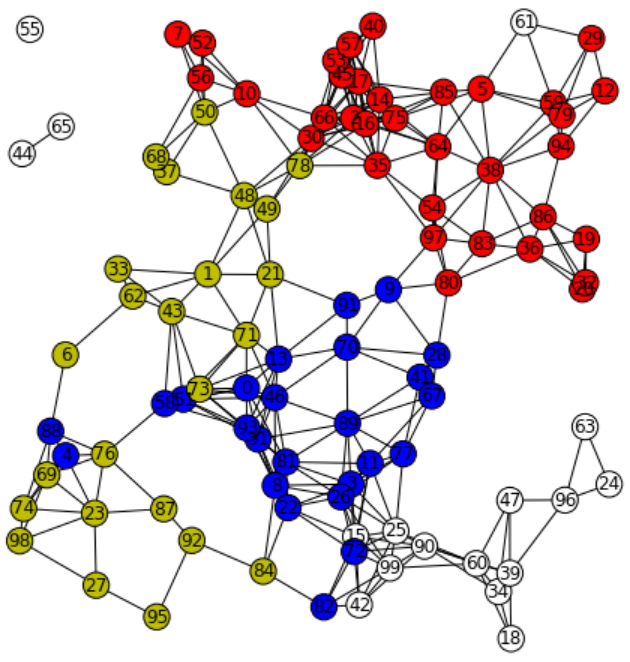
\includegraphics[width=0.33\columnwidth]{figures/fig1.png}
\end{center}
\caption{An example of a flooding algorithm being tested with the Python based NetworkX software. The graphic displays three different spreading patterns from various starting nodes according to a flooding algorithm. A simulation like this would be used to test relevant metrics of network architectures \cite{sphyce2015networkx}.}
\label{fig:2}
\end{figure}

While it is difficult to anticipate the exact network architecture that will give the best result I anticipate that routing using some form of Shortest Path Bridging healing algorithm would be best suited for this application. I anticipate that 20 nodes should be sufficient to communicate effectively with a good quality modem on the condition that the data packets sent between each node can be sufficiently compressed. I believe the packets can be sufficiently compressed with predetermined functions built into each node. I also anticipate the overall architecture will take one of two forms. The first would entail the network centered around one “master node” which operates solely to give orders to all the “worker nodes.” This would simplify data processing but leave the network more susceptible to node failure. The second would be all nodes connecting to n partners around them to communicate cooperatively and independently of a dedicated controller. This would complicate data transmission but create a more robust network. 

\section{Internship opportunity}
	This summer I will be working at a research internship with the National Geospatial Intelligence Agency. The internship will take place at the NGA headquarters in Springfield Virginia. The USNA coordinator is Prof. Andrew Muller in the USNA Oceanography Department. The NGA point of contact is Anita Clegg, the academic program manager for NGA research. The internship will last for approximately six weeks during zero and first training blocks. This internship is funded by the NGA and the United States Naval Academy.
	
Geospatial Intelligence primarily concerns deriving intelligence from imagery and analysis of geographic and hydrographic features. I will use this opportunity to research this project in terms of its relation to the collection and processing of Geospatial Intelligence. During the internship I will work with the team responsible for research and development of unmanned systems such as drones and remotely piloted aircraft. I hope to use my experience researching unmanned platforms to incorporate new ideas and capabilities relating to an unmanned mesh network into my research. In addition, I hope to gain a greater understanding of coding and control of unmanned systems as well as the physical design of the plants and sensors that allow the systems to operate and gather intelligence.

\section{Immediate Graduate School Plan}
My Immediate Graduate School Plan is to apply to the Naval Postgraduate School (NPS). The degree that I would like to pursue is Electrical/Electronic Systems Engineering (5300I) with a focus on  Sensor System Engineering. With research focused on areas such as submarine electromagnetic signatures and shielding, electronic warfare and sonar systems, and underwater acoustic propagation, this area of study at NPS would provide me with many technical expertise useful to the submarine force. I would also like to pursue this area of study because having a technical understanding of electronic systems and sensors would be extremely useful for researching and utilizing autonomous systems, an area of great interest for me. Studying this field will equip me with the necessary expertise to utilize autonomous systems as well as provide me with the necessary research skills and technical experience to aid in the development and tasking of such systems.

\section{Integration}
	If I am fortunate enough to earn a spot as a Bowman Scholar I am certain the opportunity will enable me to pursue an education and a career that will help me to serve more effectively as an officer in the submarine force. I firmly believe that a developing need in our society and more specifically in our military is the emergence of new autonomous systems both in the civilian and military domains. As a Robotics and Control Engineer I study how autonomous systems work and what they can be applied to. Autonomous systems have long been an important tool in our military’s arsenal and their relevance is only growing. The US Military is turning to autonomous systems that are faster, stealthier, and more accurate than their manned counterparts. The United States is not the only power developing and utilizing such capabilities. Potential adversaries such as Russia, China, and Iran are making great leaps in the technological capabilities of their unmanned vehicles. During my time in the military I want to help our nation develop the capability to fully take advantage of these exciting new systems. I also want to help our nation be ready to defend against similar capabilities possessed by any adversary. While my current studies are providing me with a foundational understanding of Engineering, I would like to delve deeper into the field. The ability to pursue a research project relevant to my interests and related to a developing need of the Navy through the Bowman program would be a fantastic way to explore research and gain practical engineering experience while at the Naval Academy. After completing my engineering undergraduate studies and receiving my commission as an officer, I want to continue pursuing education in the field of Electrical/Electronic Systems Engineering at the Naval Postgraduate School. I would like to pursue this field since it can readily be applied to robotic vehicles and drones capable of operating under and on the sea or in the air. Such research is what the Navy is in need of for the development of new and competitive weapons systems. I want to gain a deeper engineering proficiency and I want to learn the methods that will help me to be successful as a researcher during my time at NPS. As a submarine officer I want to serve in the capacity of a leader and an administrator while utilizing the technical education I have received to better apply the resources and weapons systems possessed by the Navy. I also eventually hope to apply what I learn to a research and development capacity in the Navy possibly as an Engineering Duty Officer. In this role I would not only utilize cutting edge technologies employed by the Navy, I would have an active role in researching and developing them as well. The Navy will undoubtedly evolve into a branch that utilizes to a major extent unmanned ships, submarines, and aircraft and I want to be equipped to provide the research skills and technical expertise that will help to usher in this evolution of the Naval Service. The Bowman program would afford me that unique opportunity. 
	
\bibliography{stites.bib}
\end{document}
